% ============================================================
%  DTSG — A0 landscape conference poster
%  build:  pdflatex dtsg_poster.tex
%  assets: architecture.png (required), igdtuw-logo.jpg (optional)
% ============================================================
\documentclass[final]{beamer}

\usepackage[orientation=landscape,size=a0,scale=1.0]{beamerposter}

\usepackage{graphicx}
\usepackage{tikz}
\usetikzlibrary{positioning,arrows.meta,calc,shapes.geometric}
\usepackage{amsmath,amssymb}
\usepackage{booktabs}
\usepackage{array}
\usepackage{ragged2e}
\usepackage{enumitem}
\usepackage{xcolor}
\usepackage[most]{tcolorbox}

% ------------------------------------------------------------
%  palette — one green, one gold, one ink, three tints
% ------------------------------------------------------------
\definecolor{IGGreen}{HTML}{005F32}   % brand green, headings and rules
\definecolor{IGDeep}{HTML}{00301A}    % darkest green, header band
\definecolor{IGMark}{HTML}{0B7A45}    % green for chart marks
\definecolor{IGGold}{HTML}{BE911E}    % accent
\definecolor{GoldMark}{HTML}{C08A2A}  % gold for chart marks
\definecolor{IGTint}{HTML}{EDF5F0}    % green tint fill
\definecolor{GoldTint}{HTML}{FBF5E4}  % gold tint fill
\definecolor{Ink}{HTML}{1E2321}       % body text
\definecolor{Muted}{HTML}{5C6360}     % secondary text
\definecolor{Hair}{HTML}{C9D4CD}      % hairlines

\setbeamercolor{normal text}{fg=Ink}
\usebeamercolor[fg]{normal text}
\setbeamertemplate{navigation symbols}{}
\setlist[itemize]{label=\textcolor{IGGold}{\rule[0.25ex]{0.45em}{0.45em}},
                  leftmargin=1.2cm, labelsep=6mm}
\setlength{\parindent}{0pt}

% ------------------------------------------------------------
%  type scale — five sizes, used consistently
% ------------------------------------------------------------
\newcommand{\Title}{\fontsize{68}{76}\selectfont}
\newcommand{\Hero}{\fontsize{54}{58}\selectfont}
\newcommand{\Lead}{\fontsize{26}{32}\selectfont}
\newcommand{\Body}{\fontsize{20}{26}\selectfont}
\newcommand{\Small}{\fontsize{17}{22}\selectfont}

\newcommand{\key}[1]{{\color{IGGreen}\bfseries #1}}
\newcommand{\gold}[1]{{\color{IGGold}\bfseries #1}}

% ------------------------------------------------------------
%  boxes — one base style, three variants
% ------------------------------------------------------------
\tcbset{
  posterbase/.style={
    enhanced, sharp corners=downhill, arc=6pt,
    boxrule=0pt, frame hidden,
    borderline west={7pt}{0pt}{IGGreen},
    colback=white,
    left=14mm, right=12mm, top=9mm, bottom=9mm,
    toptitle=4mm, bottomtitle=4mm,
    fonttitle=\bfseries\fontsize{27}{31}\selectfont,
    coltitle=white, colbacktitle=IGGreen,
    attach boxed title to top left={xshift=-7pt, yshift=0pt},
    boxed title style={sharp corners=downhill, arc=6pt, boxrule=0pt,
                       left=14mm, right=10mm, top=4mm, bottom=4mm},
  }
}

\newtcolorbox{sect}[1]{posterbase, title={#1}}

% callout: quiet tinted panel, no title bar
\newtcolorbox{panel}[1][IGTint]{
  enhanced, arc=6pt, boxrule=0pt, frame hidden,
  colback=#1, left=8mm, right=8mm, top=6mm, bottom=6mm}

% the one loud element on the poster
\newtcolorbox{headline}{
  enhanced, arc=6pt, boxrule=3pt, colframe=IGGold,
  colback=GoldTint, left=8mm, right=8mm, top=7mm, bottom=7mm}

% ------------------------------------------------------------
%  small components
% ------------------------------------------------------------
% a flow chip used in the pipeline diagrams
\tikzset{
  chip/.style={draw=IGGreen, line width=1.6pt, fill=white, rounded corners=6pt,
               align=center, inner sep=6mm, font=\fontsize{19}{23}\selectfont},
  chipfill/.style={chip, fill=IGTint},
  chipgold/.style={chip, draw=IGGold, fill=GoldTint},
  flow/.style={-{Latex[length=6mm,width=4mm]}, line width=2.2pt, IGGreen},
}

\begin{document}
\begin{frame}[t]

% ============================================================
%  HEADER — full-bleed band, logo left, title centred
% ============================================================
\begin{tikzpicture}[remember picture, overlay]
  \fill[IGDeep] (current page.north west)
    rectangle ([yshift=-13.4cm]current page.north east);
  \fill[IGGold] ([yshift=-13.4cm]current page.north west)
    rectangle ([yshift=-13.9cm]current page.north east);

  \node[anchor=west, inner sep=0pt]
    at ([xshift=4cm, yshift=-6.7cm]current page.north west) {%
      \IfFileExists{igdtuw-logo.jpg}
        {\includegraphics[height=8.6cm]{igdtuw-logo.jpg}}
        {\color{white!12}\rule{8.6cm}{8.6cm}}};

  \node[anchor=center, align=center, text width=88cm]
    at ([yshift=-6.9cm]current page.north) {%
      {\color{white}\Title\bfseries
       DTSG: A Dynamic Temporal State Graph for Agent Memory\par}
      \vspace{0.45cm}
      {\color{white}\Lead
       Gungun Jain \quad\textperiodcentered\quad Krati Mishra
       \quad\textperiodcentered\quad Sneha\par}
      \vspace{0.2cm}
      {\color{IGGold}\fontsize{22}{26}\selectfont\bfseries
       Department of Information Technology \quad\textperiodcentered\quad
       Indira Gandhi Delhi Technical University for Women\par}};
\end{tikzpicture}

\vspace*{15.2cm}

% ============================================================
%  THESIS STRIP — the poster's one-sentence argument
% ============================================================
\begin{center}
\begin{minipage}{0.965\textwidth}
\begin{tcolorbox}[enhanced, arc=6pt, boxrule=0pt, frame hidden,
  colback=IGTint, borderline west={9pt}{0pt}{IGGold},
  left=12mm, right=12mm, top=8mm, bottom=8mm]
\centering\fontsize{27}{34}\selectfont
An agent's memory is not a pile of text — it is a set of claims that
\emph{change}. DTSG stores \key{what was said} apart from \key{what is still
true}, and ranks by \key{relevance $\times$ validity $\times$ recency}.
\end{tcolorbox}
\end{minipage}
\end{center}

\vspace{0.9cm}

% ============================================================
\begin{columns}[t, totalwidth=0.965\textwidth, onlytextwidth]

% ============================================================
%  COLUMN 1 — problem and idea
% ============================================================
\begin{column}{0.280\textwidth}

\begin{sect}{1\quad The problem}
\Body\justifying
Retrieval-augmented memory ranks by semantic similarity alone. When a fact is
updated, the old and the new sentence are \emph{about the same thing}, so they
embed almost identically.

\vspace{0.7cm}
\centering
\begin{tikzpicture}
  \node[chipfill, minimum width=13cm] (old)
    {\textbf{``I live in Delhi''}\\[1mm]{\Small\color{Muted}stated Jul 2025}};
  \node[chipgold, minimum width=13cm, below=2.4cm of old] (new)
    {\textbf{``I moved to Berlin''}\\[1mm]{\Small\color{Muted}stated May 2026}};
  \draw[flow] (old) -- node[right=2mm, font=\fontsize{18}{20}\selectfont]
    {knowledge update} (new);
\end{tikzpicture}

\vspace{0.7cm}
\begin{panel}[GoldTint]
\centering\Lead
Similarity says what is \emph{relevant}.\\
It cannot say what is \gold{true now}.
\end{panel}

\vspace{0.6cm}
\justifying\Body
\begin{itemize}[leftmargin=*, itemsep=4mm]
  \item Which of the two lands on top is decided by noise, not by truth.
  \item The agent does not hedge — it states the stale answer confidently.
  \item Deleting the old fact fixes ranking but destroys history.
\end{itemize}
\end{sect}

\vfill

\begin{sect}{2\quad The idea}
\Body\justifying
Split memory by mutability: an append-only log of what was said, and a graph of
what currently holds.

\vspace{0.7cm}
\centering
\begin{tikzpicture}
  \node[chipfill, minimum width=13cm, minimum height=5cm] (log)
    {\textbf{IMMUTABLE EVENT LOG}\\[1.5mm]{\Small\color{Muted}every message, never rewritten}};
  \node[chipgold, minimum width=13cm, minimum height=5cm, below=2.6cm of log] (graph)
    {\textbf{TEMPORAL STATE GRAPH}\\[1.5mm]{\Small\color{Muted}subject--predicate--object facts}};
  \draw[flow] (log) -- node[right=2mm, font=\fontsize{18}{20}\selectfont] {derives} (graph);
\end{tikzpicture}

\vspace{0.7cm}
\justifying\Body
Each fact carries a \key{status}, a \key{validity interval} and a
\key{supersede link}. A contradicted fact is marked \key{EXPIRED} and pointed at
its replacement — never deleted, so history stays queryable.
\end{sect}

\vfill

\begin{sect}{3\quad Nothing is deleted}
\centering
\begin{tikzpicture}[x=1cm, y=1cm]
  \node[chipfill, minimum width=7cm, minimum height=3.2cm] (d) at (0,0) {\textbf{Delhi}};
  \node[chipfill, minimum width=7cm, minimum height=3.2cm, right=2.2cm of d] (b) {\textbf{Berlin}};
  \node[chipgold, line width=3pt, minimum width=7cm, minimum height=3.2cm, right=2.2cm of b] (l) {\textbf{Lisbon}};
  \draw[flow] (d) -- (b);
  \draw[flow] (b) -- (l);
  \node[above=2mm of d, font=\fontsize{16}{19}\selectfont\bfseries, Muted] {EXPIRED};
  \node[above=2mm of b, font=\fontsize{16}{19}\selectfont\bfseries, Muted] {EXPIRED};
  \node[above=2mm of l, font=\fontsize{16}{19}\selectfont\bfseries, IGGold] {ACTIVE};
  \node[below=2mm of d, font=\fontsize{14}{17}\selectfont, Muted] {Jul 25 $\rightarrow$ May 26};
  \node[below=2mm of b, font=\fontsize{14}{17}\selectfont, Muted] {May 26 $\rightarrow$ Aug 26};
  \node[below=2mm of l, font=\fontsize{14}{17}\selectfont, Muted] {Aug 26 $\rightarrow$ now};
\end{tikzpicture}

\vspace{0.6cm}
\justifying\Body
Rows are joined by \texttt{superseded\_by}. Two moves produce three rows, not
one overwrite — so \emph{``where did I live last spring?''} stays answerable
from the same store.
\end{sect}

\end{column}

% ============================================================
%  COLUMN 2 — how it works
% ============================================================
\hspace{0.012\textwidth}
\begin{column}{0.378\textwidth}

\begin{sect}{4\quad Architecture}
\centering
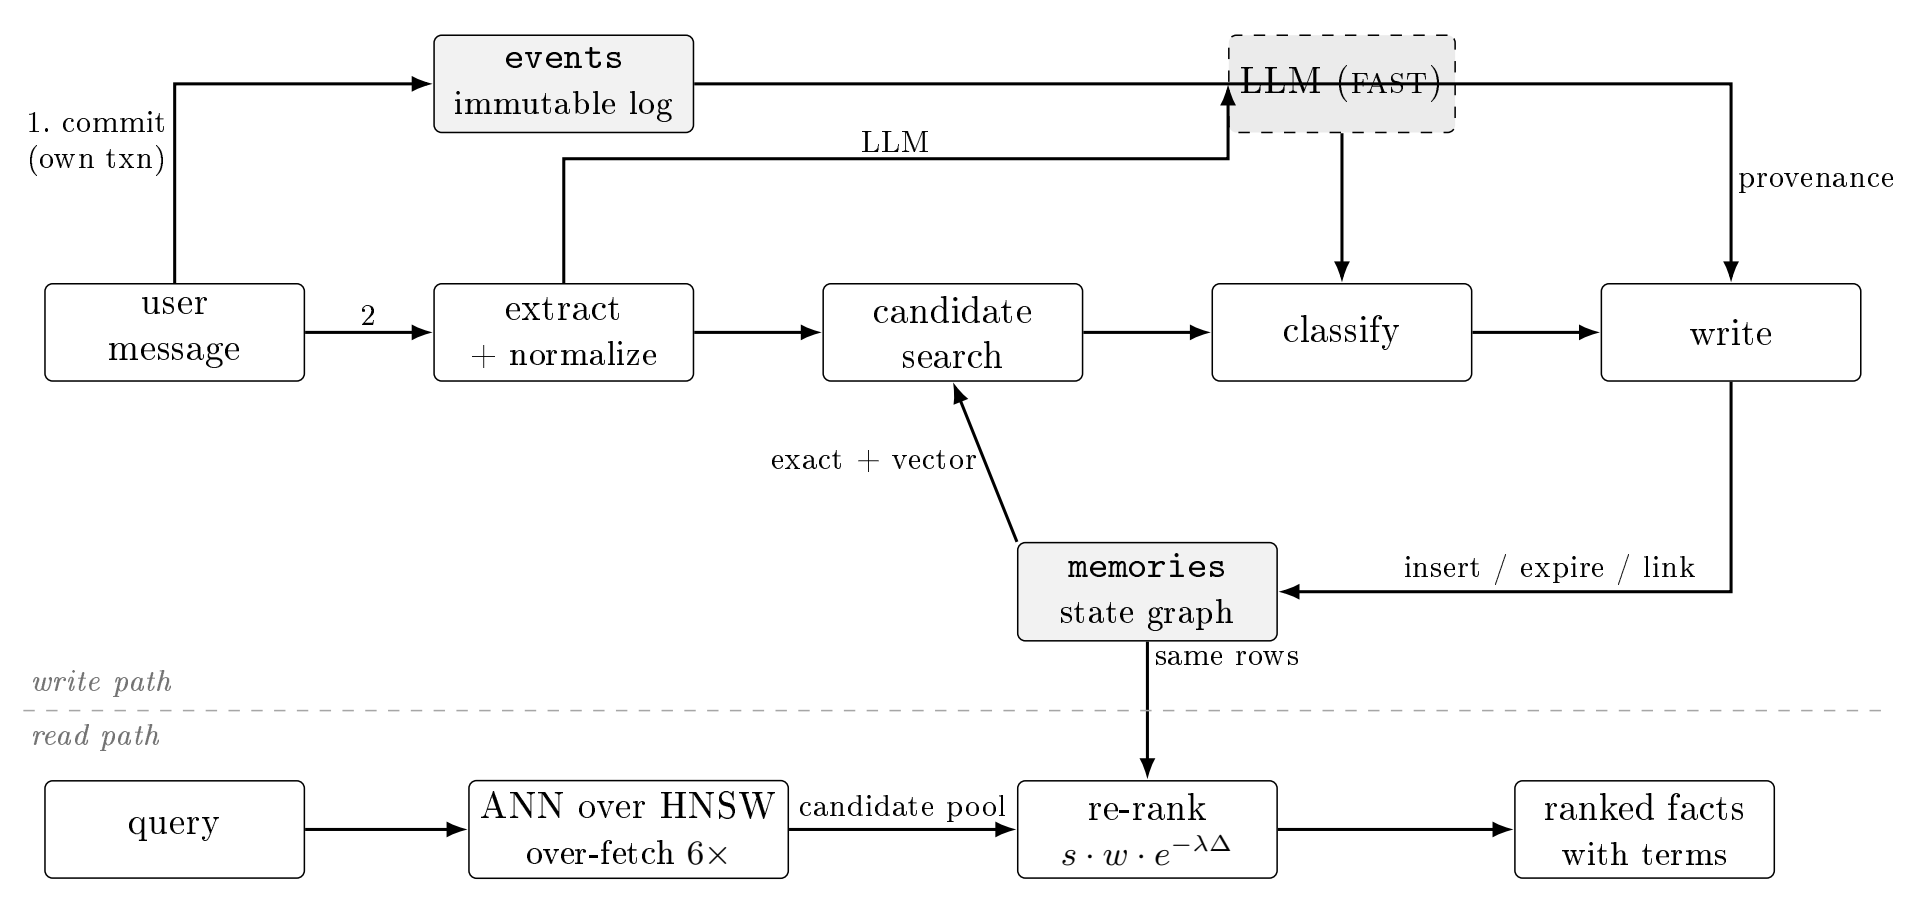
\includegraphics[width=\linewidth]{architecture.png}

\vspace{0.5cm}
\begin{minipage}{\linewidth}
{\Small\color{Muted}\raggedright
\textbf{Figure 1.} The write path commits the raw message first, in its own
transaction, before any derived state. The read path over-fetches from the HNSW
index and re-ranks in Python. Dashed nodes are language-model calls.\par}
\end{minipage}
\end{sect}

\vfill

\begin{sect}{5\quad Write path}
\centering
\begin{tikzpicture}[node distance=1.6cm]
  \node[chipfill] (m) {USER\\MESSAGE};
  \node[chip, right=of m] (e) {EXTRACT\\+ NORMALIZE};
  \node[chip, right=of e] (c) {CANDIDATE\\SEARCH};
  \node[chip, right=of c] (l) {LLM\\CLASSIFY};
  \node[chipfill, right=of l] (w) {WRITE\\STATE};
  \draw[flow] (m) -- (e); \draw[flow] (e) -- (c);
  \draw[flow] (c) -- (l); \draw[flow] (l) -- (w);
\end{tikzpicture}

\vspace{0.8cm}
\justifying\Body
\textbf{Normalization} folds every first-person subject to \texttt{user},
snake-cases predicates, and maps \key{22 surface variants onto 15 canonical
predicates} — without it, \texttt{lives\_in} and \texttt{resides\_in} never
match and contradictions go undetected.

\vspace{0.6cm}
\textbf{Candidate search} runs two arms: an \key{exact} match on
subject\,+\,predicate, always included, and a \key{vector} arm above a 0.55
similarity floor. The classifier resolves the new fact against them:

\vspace{0.5cm}
{\Body
\begin{tabular}{@{}p{7.5cm}@{\hspace{6mm}}p{22.5cm}@{}}
\toprule
\textbf{\color{IGGreen}REINFORCE} & the fact restates a held one — raise its
confidence, store no copy \\[3mm]
\textbf{\color{IGGreen}ADDITIVE} & the fact coexists — store it, touch nothing \\[3mm]
\textbf{\color{IGGold}SUPERSEDE} & the fact contradicts — store it, expire and
link the old \\
\bottomrule
\end{tabular}}

\vspace{0.5cm}
\justifying\Body
The judgement that matters is \key{additive vs.\ supersede} — whether a
predicate can hold several values at once. \emph{Speaks} can; \emph{lives in}
cannot. Nothing in the schema decides it, so the model is asked, and told to
choose the recoverable error when unsure.
\end{sect}

\vfill

\begin{sect}{6\quad Read path: temporal ranking}
\centering
{\fontsize{34}{40}\selectfont
\[
  S(q,f)\;=\;\underbrace{\operatorname{sim}(q,f)}_{}
  \;\times\;\underbrace{w_{\text{status}}(f,t)}_{}
  \;\times\;\underbrace{e^{-\lambda\,\Delta t}}_{}
\]}
\vspace{-0.4cm}

{\Body
\begin{tabular}{@{}p{9.5cm}p{10cm}p{9.5cm}@{}}
\key{relevance} & \key{validity} & \key{recency}\\
cosine over embeddings & evaluated \emph{at query time} & 180-day half-life
\end{tabular}}

\vspace{0.7cm}
\justifying\Body
The status term is read against the query's reference time, not from the stored
column — so \emph{``where do I live?''} and \emph{``where did I live in March?''}
are the same query with a different $t$, answered from one store.
\end{sect}

\end{column}

% ============================================================
%  COLUMN 3 — evidence
% ============================================================
\hspace{0.012\textwidth}
\begin{column}{0.280\textwidth}

\begin{sect}{7\quad Results}
\Small\color{Muted}\justifying
Four hand-built cases in which the \emph{stale} fact is the equal-or-better
textual match — the situation where cosine-only retrieval cannot be right by
accident. Cases carry their own similarity scores, so no embedding model enters
the comparison.

\vspace{0.8cm}
\centering
% ---- grouped bars: DTSG vs naive RAG -----------------------
\begin{tikzpicture}[x=1cm, y=1cm]
  \useasboundingbox (-0.6,-6.2) rectangle (16.4,10.4);
  \def\bw{2.2}          % bar width
  \def\h{9}             % full-scale height
  % one baseline; the bars are directly labelled, so no axis is needed
  \draw[Hair, line width=1.5pt] (-0.4,0) -- (16.2,0);
  % group 1 — correct current fact (3/3 vs 0/3)
  \fill[IGMark, rounded corners=5pt] (0.9,0) rectangle (0.9+\bw,\h);
  \node[font=\fontsize{20}{22}\selectfont\bfseries, IGMark, above]
    at (0.9+\bw/2,\h+0.15) {3/3};
  \node[font=\fontsize{16}{18}\selectfont, Muted, above] at (3.9+\bw/2,0.15) {0/3};
  \draw[GoldMark, line width=2pt] (3.9,0) -- (3.9+\bw,0);
  % group 2 — stale top hit (0/4 vs 3/4)
  \node[font=\fontsize{16}{18}\selectfont, Muted, above] at (8.9+\bw/2,0.15) {0/4};
  \draw[IGMark, line width=2pt] (8.9,0) -- (8.9+\bw,0);
  \fill[GoldMark, rounded corners=5pt] (11.9,0) rectangle (11.9+\bw,0.75*\h);
  \node[font=\fontsize{20}{22}\selectfont\bfseries, GoldMark, above]
    at (11.9+\bw/2,0.75*\h+0.15) {3/4};
  % group labels
  \node[align=center, font=\fontsize{18}{21}\selectfont, below] at (3.9,-0.5)
    {\textbf{Correct current fact}\\[1mm]{\color{Muted}higher is better}};
  \node[align=center, font=\fontsize{18}{21}\selectfont, below] at (11.9,-0.5)
    {\textbf{Stale fact on top}\\[1mm]{\color{Muted}lower is better}};
  % legend
  \fill[IGMark, rounded corners=3pt] (2.6,-4.6) rectangle (3.5,-4.0);
  \node[right, font=\fontsize{18}{21}\selectfont] at (3.7,-4.3) {DTSG};
  \fill[GoldMark, rounded corners=3pt] (8.6,-4.6) rectangle (9.5,-4.0);
  \node[right, font=\fontsize{18}{21}\selectfont] at (9.7,-4.3) {Naive RAG};
\end{tikzpicture}

\vspace{0.7cm}

\begin{headline}
\centering
{\Hero\bfseries\color{IGGreen}3/3\quad vs\quad 0/3}\\[3mm]
{\Lead DTSG picks the current fact in every scored case;\\
the cosine-only baseline in none — and never tops a stale fact.}
\end{headline}
\end{sect}

\vfill

\begin{sect}{8\quad Which term does the work?}
\Small\color{Muted}\justifying
A controlled scenario: the user moved from Delhi to Berlin 10 days ago and both
facts have cosine similarity \emph{exactly} 1.000, so a vector store cannot
distinguish them even in principle.

\vspace{0.6cm}
\centering\color{Ink}
{\Body
\begin{tabular}{@{}l l r r@{}}
\toprule
\textbf{Fact} & \textbf{Status} & \textbf{sim.} & \textbf{score}\\
\midrule
Berlin & \color{IGGreen}\textbf{ACTIVE} & 1.000 & \textbf{0.9622}\\
Delhi  & \color{Muted}EXPIRED & 1.000 & 0.1443\\
\midrule
\multicolumn{4}{@{}l@{}}{\Small\itshape asked \texttt{as\_of} 60 days ago, the order inverts:}\\
Delhi  & \color{IGGreen}\textbf{held then} & 1.000 & \textbf{1.0000}\\
Berlin & \color{Muted}not yet true & 1.000 & 0.1500\\
\bottomrule
\end{tabular}}

\vspace{0.7cm}
\justifying\Body
With decay switched off the separation still holds — the \key{status weight},
not recency, is what divides live from dead. And it is a discount, not a filter:
raising $w_{\text{exp}}$ brings the old fact back for \emph{``where have I
lived?''}
\end{sect}

\vfill

\begin{sect}{9\quad Conclusion}
\centering
{\Hero\bfseries\color{IGGreen}103}\\[1mm]
{\Lead automated tests passing}\\[2mm]
{\Small\color{Muted}extraction \textperiodcentered\ normalization \textperiodcentered\
immutability \textperiodcentered\ transactions \textperiodcentered\ chain walking
\textperiodcentered\ ranking}

\vspace{0.8cm}
\justifying\Body
Choosing between an old fact and its replacement is a \key{write-time problem
wearing a read-time disguise}: the information needed is the record of which one
replaced the other. DTSG writes that record down and spends it at read time.

\vspace{0.6cm}
{\Small\color{Muted}\justifying
\textbf{Next:} validate extraction and classification against a live model;
evaluate on the knowledge-update subsets of LongMemEval and LoCoMo; learn
per-predicate half-lives; entity resolution over objects; multi-hop retrieval.}
\end{sect}

\end{column}
\end{columns}

% ============================================================
%  FOOTER
% ============================================================
\vfill
\begin{tikzpicture}[remember picture, overlay]
  \fill[IGGold] ([yshift=2.6cm]current page.south west)
    rectangle ([yshift=2.9cm]current page.south east);
  \fill[IGDeep] (current page.south west)
    rectangle ([yshift=2.6cm]current page.south east);
  \node[anchor=center, text=white, font=\fontsize{21}{25}\selectfont]
    at ([yshift=1.3cm]current page.south) {%
      ACM Research Summer Internship 2026 \quad\textperiodcentered\quad
      Department of Information Technology \quad\textperiodcentered\quad IGDTUW};
\end{tikzpicture}

\end{frame}
\end{document}
